\section{JUnit-Tests}
This part is at least as important as the code itself. Indeed, it is impossible to write a computer program without making mistakes. They can be found and corrected only by running tests. In our software, we chose to use JUnit-Tests.

\subsection{Why use JUnit-Tests?}
\label{sub:why_use_JUnih-Tests}

Using JUnit is much more convenient than writing tests in a main method, for several reasons: JUnit-tests allow to check \textit{independently} whether each unit of code works or does not. Moreover, while tests made in main methods are non-reproductible and hard to understand, JUnit-Tests can be \textit{documented} and therefore explained, and they can be executed whenever required (totally \textit{reproductible}). This means that every change in the existing code can be checked by simply running the tests which already exist.

\subsection{Test organisation}
\label{sub:test_organisation}

In order to have efficient tests, we chose to separate the writing of the code and the tests: one of us wrote some parts of the program and the other one tested it. Doing so enables findind much more errors because the tester does not know how the code works but is only aware of the desired results. Thus, some tests the code writer would have never thought to do can be implemented.
Furthermore, all the tests have been distributed so that those which test the same package are put together:
\begin{itemize}
	\item{\textbf{testrestaurant}} Contains all the tests of the \textit{restaurant} package.
	\item{\textbf{testSystem}} Contains all the tests of the  \textit{system} package.
	\item{\textbf{test\_Usermanagement}} Contains all the tests of the \textit{user\_management} package.
\end{itemize}
Each package holds classes, and each of them contains the tests of one class. For instance, the class called \textit{TestMyFoodora} in the package \textit{testSystem} holds all the tests of the class \textit{MyFoodora}.  
Note that there is no test for the packages \textit{commandLineTool}, \textit{GUI} and \textit{scenario}. The reasons are as follows:
\begin{itemize}
	\item{\textit{commandLineTool}} package contains the Command-Line User Interface. It is not possible to test it with JUnit-Tests because running it needs to input command lines in the console. Nevertheless, it can be tested thanks to the command line "runtest" which runs an input file or a default file if no input file is given.
	\item{\textit{GUI}} package contains the Graphical User Interface. We did not find a way to test it other than doing it by hand by using the mouse.
	\item{\textit{scenario}} package contains scenarios which test the software.
\end{itemize}

\subsection{Problems solved}
\label{sub:problems_solved}

\begin{comment}
copy paste errors


use of exception in tests to test if the exception is thrown as excepted (for example: testDesertAndStarter)

round problem: how was it solved ? Don't remember, maybe problems in computation
\end{comment}
Several errors have been solved thanks to JUnit-Tests, as follows:
\begin{itemize}
	\item{\textit{testAddItemToMealDoesNotExist}} in the class \textit{MealTest} showed that there was no exception handled when a user tried to add an item to a meal which does not exist. That is why a throw of the excpetion \textit{WrongItemAdded} has been added to the method \textit{Menu.addItem}, which is caught later in the program and therefore allows to display a message without stopping the program.
	\item{\textit{testDifferentID}} showed that every meal or single item had the same IDs. A static counter has been added to the attributes of \textit{Meal} and \textit{SingleItem}, which is incremented each time a new instance is created.
	\item{\textit{tests of the fidelity card setting}} in the class \textit{TestCustomer} showed that it was possible to set a new fidelity card only if the old one was a point fidelity card. Indeed, in the method \textit{Customer.setFidelityCard}, there was:
\lstinputlisting[firstline=5,lastline=17]{./Code/src/Code/FidelityCardCode.java}
As showed in the previous code, there was a \textit{if condition} to display the message \textit{"You will lose all your points."}, but inadvertently all the conditions \textit{name.equalsIgnoreCase(...)} were put inside the first \textit{if}, not outside.
	\item{} copy-paste errors have been corrected thanks to JUnit-Tests as well.
\end{itemize}
Note that the choice of using exceptions is very useful in JUnit-Tests to check when a case is expected to fail. Indeed, instead of having tests which voluntarily fail, the tests can succeed if the exception is caught. For instance:
\lstinputlisting[firstline=45,lastline=62]{./../src/testrestaurant/MealTest.java}


\subsection{Use of the plugin \textit{EclEmma}}
\label{sub:use_of_the_plugin_EclEmma}

In order to know how much of the program had been tested by the JUnit-Tests, we used a plugin called \textit{EclEmma}. For each test executed, it gives the percentage of the program which has been tested for each package, as illustrated in the next figure. 
\begin{figure}[H]
	\centering
	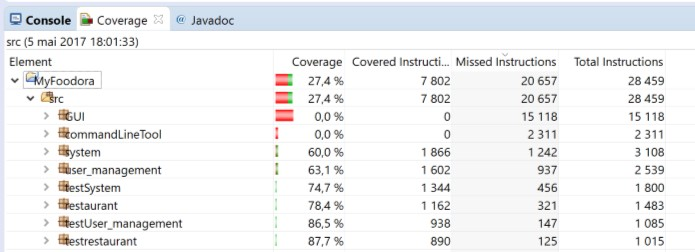
\includegraphics[width=1\linewidth]{./ima/testcoverage.jpg}
	\caption{Test coverage}
	\label{fig:test-coverage}
\end{figure}
As illustrated in the figure, the first column of the chart shows the coverage percentage of the code which is tested by the JUnit-Tests. One can notice that:
\begin{itemize}
	\item{} The packages \textit{GUI}, \textit{commandLineTool} and \textit{scenario} are not tested (see explication \ref{sub:test_organisation}).
	\item{} The total coverage is just 26.7\% because the packages \textit{GUI}, \textit{commandLineTool} and \textit{scenario} represent more than half of the code.
	\item{} All of the packages \textit{user\_management}, \textit{system} and \textit{restaurant} are tested at more than 60\% (even 78\% for \textit{restaurant}). Actually, the plugin takes into account the getters and setters which are not necessarily used during the tests, which means that the core of the classes are tested at more than 60\%.
	\item{} The packages \textit{testSystem}, \textit{testUser\_management} and \textit{testRestaurant} are not fully tested because the tests contain \textit{catch} blocks which are not executed while running them.
\end{itemize}
Moreover, after running the JUnit-Tests with this plugin, all the code lines are highlighted in green, yellow or red as illustrated in the next figure.
\begin{figure}[H]
	\centering
	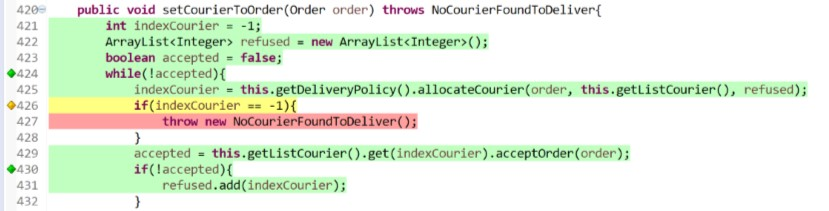
\includegraphics[width=1\linewidth]{./ima/testlinecolor.jpg}
	\caption{Highlighting of the code line after the tests with the plugin}
	\label{fig:line-test-plugin}
\end{figure}
The lines are highlighted in green when the code executes them, and in red if it does not. A line is yellow if some of the conditions have been missed: in the previous figure, 1 of the 2 conditions has been missed. Indeed, \textit{indexCourier} is different from -1 so the false-case has been checked but not the true one. \textbf{This highlighting is very useful because it helps to know what tests have not been implemented yet.}